\section{Erzeugende Muster}
\label{sec:Kap-10.1}

\textit{Erzeugende Muster} abstrahieren den Instanziierungsprozess und machen eine Anwendungssoftware unabhängig davon, wie ihre Objekte erzeugt und zusammen\-gesetzt werden. Erzeugende Muster werden dann wichtig, wenn die Software nach einigen Änderungen immer mehr auf die Komposition vieler Objekte als auf wenige Generalisierungshierarchien aufbaut.
%Im Verlauf der Evolution von Anwendungssystemen wird es nämlich erfahrungsgemäß immer wichtiger, den Fokus von festverdrahteten komplexen Schnittstellen hin zu einer Menge möglichst schlanker, orthogonaler Schnittstellen zu verschieben, aus denen die komplexeren Schnittstellen zusammengesetzt werden können.
Die Erzeugung von Objekten mit bestimmtem Verhalten erfordert dann mehr als die einfache Instanziierung einer Klasse.

In \cite{gam95} werden fünf erzeugende Muster vorgestellt, die teilweise aufeinander aufbauen:

\begin{description}
	\setlength{\itemsep}{2mm} %%% für Druck
	
	\item[\textit{Abstrakte Fabrik}] (abstract factory) bietet eine Schnittstelle zum Erzeugen von Familien verwandter oder voneinander abhängiger Objekte, ohne ihre konkreten Klassen zu benennen.
	\item[\textit{Einzelstück}] (singleton) stellt sicher, dass von einer Klasse nur eine einzige Instanz existiert, und bietet einen globalen Zugriffsmechanismus auf diese Instanz an.
	\item[\textit{Erbauer}] (builder) trennt den Aufbau eines komplexen Objekts von seiner Darstellung, so dass mittels desselben Konstruktionsvorgangs verschiedene Repräsentationen erzeugt werden können.
	\item[\textit{Fabrikmethode}] (factory method) definiert eine Schnittstelle zur Erzeugung eines Objekts, aber überlässt die Entscheidung, welche Klasse zu instanziieren ist, den Unterklassen. Die Fabrikmethode ermöglicht einer Klasse, die Instanzi\-ierung ihren Unterklassen zu überlassen.
	\item[\textit{Prototyp}] (prototype) spezifiziert die Art der zu erzeugenden Objekte über eine \mbox{exemplarische} Instanz und erzeugt neue Objekte durch Kopieren dieser Instanz.
\end{description}

\vspace{\baselineskip}
\textcolor{FernUni-MI-green}{\noindent\rule[1ex]{\textwidth}{2pt}}\\
{\Large \textcolor{FernUni-MI-green}{\textsc{Abstrakte Fabrik (Abstract Factory)}}}\\
\textcolor{FernUni-MI-green}{\noindent\rule[1ex]{\textwidth}{2pt}}

\begin{description}
	\setlength{\itemsep}{2mm} %%% für Druck
	
	\item[Zweck] Bietet eine Schnittstelle zum Erzeugen von Familien verwandter oder voneinander abhängiger Objekte, ohne ihre konkreten Klassen zu benennen.
	\item[Motivation] Angenommen, eine Klassenbibliothek zur Unterstützung grafisch-
	\linebreak %%% für Druck
	interaktiver Benutzungsschnittstellen soll mehrere „Look\&Feel“-Standards unterstützen, wobei unterschiedliche Standards unterschiedliches Aussehen und Verhalten von graphischen Bedienungselementen wie \zb Scrollbar oder 
	\linebreak %%% für Druck
	Fenstern festlegen. Um unter verschiedenen solcher Standards lauffähig zu sein, darf eine Anwendungssoftware die benutzten Bedienelemente nicht statisch zur Kompilierungszeit festlegen, sondern muss dynamisch zur Laufzeit die ge\-eigneten Elemente auswählen und entsprechende Klassen instanziieren.
	
\pagebreak %%% für Druck

	Wir können dieses Problem lösen, indem wir in einer abstrakten Klasse eine Schnittstelle definieren, welche Operationen zur Erzeugung jedes Bedien\-elements zur Verfügung stellt. Für jeden zu unterstützenden Standard bilden wir eine (konkrete) Unterklasse dieser abstrakten Klasse. Zusätzlich definieren wir für jedes der Bedienelemente eine abstrakte Klasse, von der für jeden Standard eine Unterklasse zur Realisierung des entsprechenden Elements abgeleitet wird. Die Erzeugungsoperation für ein Bedienelement liefert nun bei jedem Aufruf eine neue Instanz dieses Bedienelements, aber je nach gewählter konkreter Fabrik-Unterklasse eine Instanz der Element-Unterklasse, die das Bedienelement für den entsprechenden Standard realisiert.
	
	Anwendungsprogramme, welche die Elemente der Benutzungsschnittstelle verwenden erzeugen diese ausschließlich über die Schnittstelle der abstrakten Klasse und haben keinerlei Kenntnis von der konkreten Realisierung der Elemente für einen bestimmten Benutzungsschnittstellen-Standard.
	\item[Anwendbarkeit] Man verwendet das Muster Abstrakte Fabrik unter folgenden
	\linebreak %%% für Druck
	Bedingungen:
	\begin{itemize}
		\item 	Die Anwendungssoftware soll unabhängig davon sein, wie bestimmte 
		\linebreak %%% für Druck
		Objekte (im Muster „Produkte“ genannt) erzeugt, zusammengesetzt und präsentiert werden.
		\item 	Die Anwendungssoftware soll für eine von mehreren Familien von Produkten konfigurierbar sein.
		\item 	Nur Produkte aus einer Familie können zusammenarbeiten.
		\item 	Eine Bibliothek wiederverwendbarer Klassen soll nur über die Schnittstellen verfügbar gemacht werden.
	\end{itemize}
	
	\item[Struktur] Abbildung~\ref{fig:muster_abstrakte_fabrik} zeigt die allgemeine Struktur des Musters Abstrakte
	\linebreak %%% für Druck
	Fabrik.
	
	\begin{figure}[h!]
		\centering
		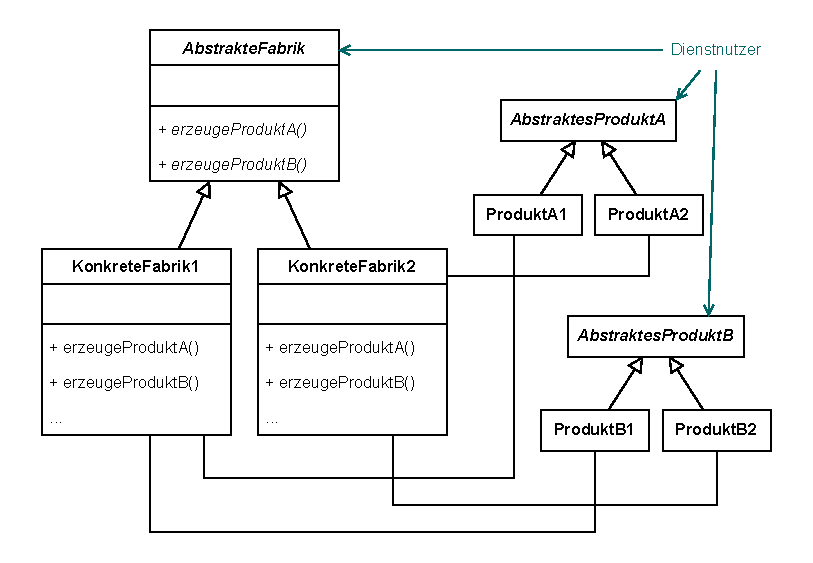
\includegraphics[scale=1.0]{Bilder/Kapitel-10/muster_abstrakte_fabrik.pdf}
		\caption{Allgemeine Struktur des Musters Abstrakte Fabrik}
		\label{fig:muster_abstrakte_fabrik}
	\end{figure}	
	
	\vspace{1mm} %%% für Druck
	
	\item[Konsequenzen] Das Muster Abstrakte Fabrik hat folgende Vor- und Nachteile:
	\begin{itemize}
		\item 	Es isoliert konkrete Klassen und hilft die von der Anwendungssoftware instanziierbaren Klassen zu kontrollieren. Da eine Fabrik die Verantwortlichkeit und den Prozess der Erzeugung von Produkt\-instanzen verkapselt, isoliert sie die Anwendungssoftware von den realisierenden Klassen. Klassennamen der konkreten Produktklassen tauchen somit nicht in den Klassen der Anwendungssoftware auf. Diese manipuliert Produkt\-instanzen nur über die Schnittstelle der abstrakten Produktklassen.
		\item 	Es vereinfacht den Austausch ganzer Produktfamilien, da die Klasse einer konkreten Fabrik nur einmal explizit angesprochen wird, nämlich am Ort ihrer Instanziierung.
		\item 	Die von der Anwendungssoftware verwendete Produktfamilie kann einfach durch Angabe einer anderen konkreten Fabrik geändert werden. 
		\item 	Es erzwingt die Konsistenz der von der Anwendungssoftware benutzten Produkte, wenn zu einem bestimmten Zeitpunkt nur genau eine Instanz (einer Unterklasse) der Klasse \sttpUMLText{AbstrakteFabrik} existieren darf. Dies ist insbesondere dann wichtig, wenn die Produkte aus unterschiedlichen Familien nicht untereinander kompatibel sind.
		\item 	Es erschwert die Hinzunahme neuer Produkte, da jede abstrakte Fabrik eine Operation zur Erzeugung jedes Produkts einer Familie definiert. Für jedes neue Produkt müssen also diese Schnittstelle und eine Implementierung in allen konkreten Unterklassen der abstrakten Fabrik sowie des abstrakten Produkts eingeführt werden.
	\end{itemize}
\end{description}
